\chapter{Quorum}
\label{cha:Results}
asdas
\iffalse
In this chapter, a framework that solely focuses on the confirmation speed of transactions is discussed. The paper discussed will be \emph{Thunderella: Blockchains with Optimistic Instant Confirmation} \cite{thunderella}. The protocol assumes that there is a secure underlying Proof-of-Work protocol such as the one described in chapter \ref{cha:pow}, but proposes a so-called optimistic fast-path for instant confirmations on transactions. As such it does not seek to solve the issues regarding the energy consumption, but only giving users faster confirmation time. The Thunderella paper describes both how the protocol can be used in a permissioned and permissionless setting. This thesis has so far only looked into the permissionless setting, and thus only this case will be further described regarding the Thunderella protocol.

% Thunderella - 
\section{Thunderella}

\subsection{Design}

The protocol consists of a designated leader and a committee, that can acknowledge transactions. Intuitively, the optimistic fast-path works in the following way.

\begin{enumerate}
    \item Transactions are sent to the leader, who signs the transactions along with a sequence number and broadcasts it to a "committee" of players.
    \item The committee members acknowledge these transactions with a response \emph{ack} to the leader, but only acknowledge one transaction per sequence number.
    \item If a transaction has more than $\frac{3}{4}$ \emph{ack}, it will be referred as \emph{notarized}. Participants can directly output their longest sequence of consecutive notarized transactions, all of which are confirmed.
\end{enumerate}

Obviously, given an honest leader and a $\frac{3}{4}$ honest committee, the described protocol works. It is efficient as it only requires one round-trip of communications, s.t., transactions can be validated quickly. The flaw here is that peers are heavily relying on the leader to act honestly and being active. As such to overcome a malicious leader, a fallback to an underlying blockchain which is much slower is used. This allows the protocol to maintain the stronger guarantees for liveness and consistency, as shown in the analysis of proof-of-work, see chapter \ref{cha:pow}. If a malicious activity is detected, a \emph{cool-down} period happens, in which both the committee and leader stops signing messages, but allow the committee to broadcast any notarized transactions they have seen so far. The length of the \emph{cool-down} period is set by \emph{some} security parameter $\kappa$. After the \emph{cool-down} period, a \emph{slow-period} happens in which transactions get confirmed as regular transactions in the underlying blockchain protocol.\\

Now there are still two things missing from the mentioned description; How a cheating action is detected and how the committee is selected.

\paragraph{Detecting Cheating} It is quite simple for a peer to see if the committee and/or leader is either cheating or inactive. If a peer notices that his transaction is not getting confirmed by a leader or the members of the committee, he can send the transaction directly to the underlying blockchain. If the peer sees some transaction on the blockchain that has not been notarized after some time interval, the member knows that the leader or a sufficient amount of the members in the committee must be cheating or unavailable. Upon detecting this the leader and the committee should enter the \emph{cool-down} period as described previously. The leader also cannot be falsely accused as the leader can confirm transactions before $n$ blocks are created on the underlying blockchain.

\paragraph{Selecting the committee} \cite{thunderella} considers two approaches to selecting a committee. One where all the parties are used in the committee and another where only the recent miners are used in the committee. As using all the parties, described in a permissionless setting is infeasible, \cite{thunderella} proposes the alternative that given it is a cryptocurrency, a set of stakeholders in the system will be selected as the committee and leader. The latter approach, where the recent miners are used in the committee, the underlying blockchain has to be \emph{fair} such that the fraction of honestly mined blocks is close to the fraction of honest parties in the network. \cite{thunderella} notes that the paper \emph{Fruitchains: A fair blockchain} shows that every blockchain can be turned into a \emph{fair} one, and thereby the requirement of a \emph{fair} blockchain is not a concern. 

\begin{figure}[H]
    \centering
    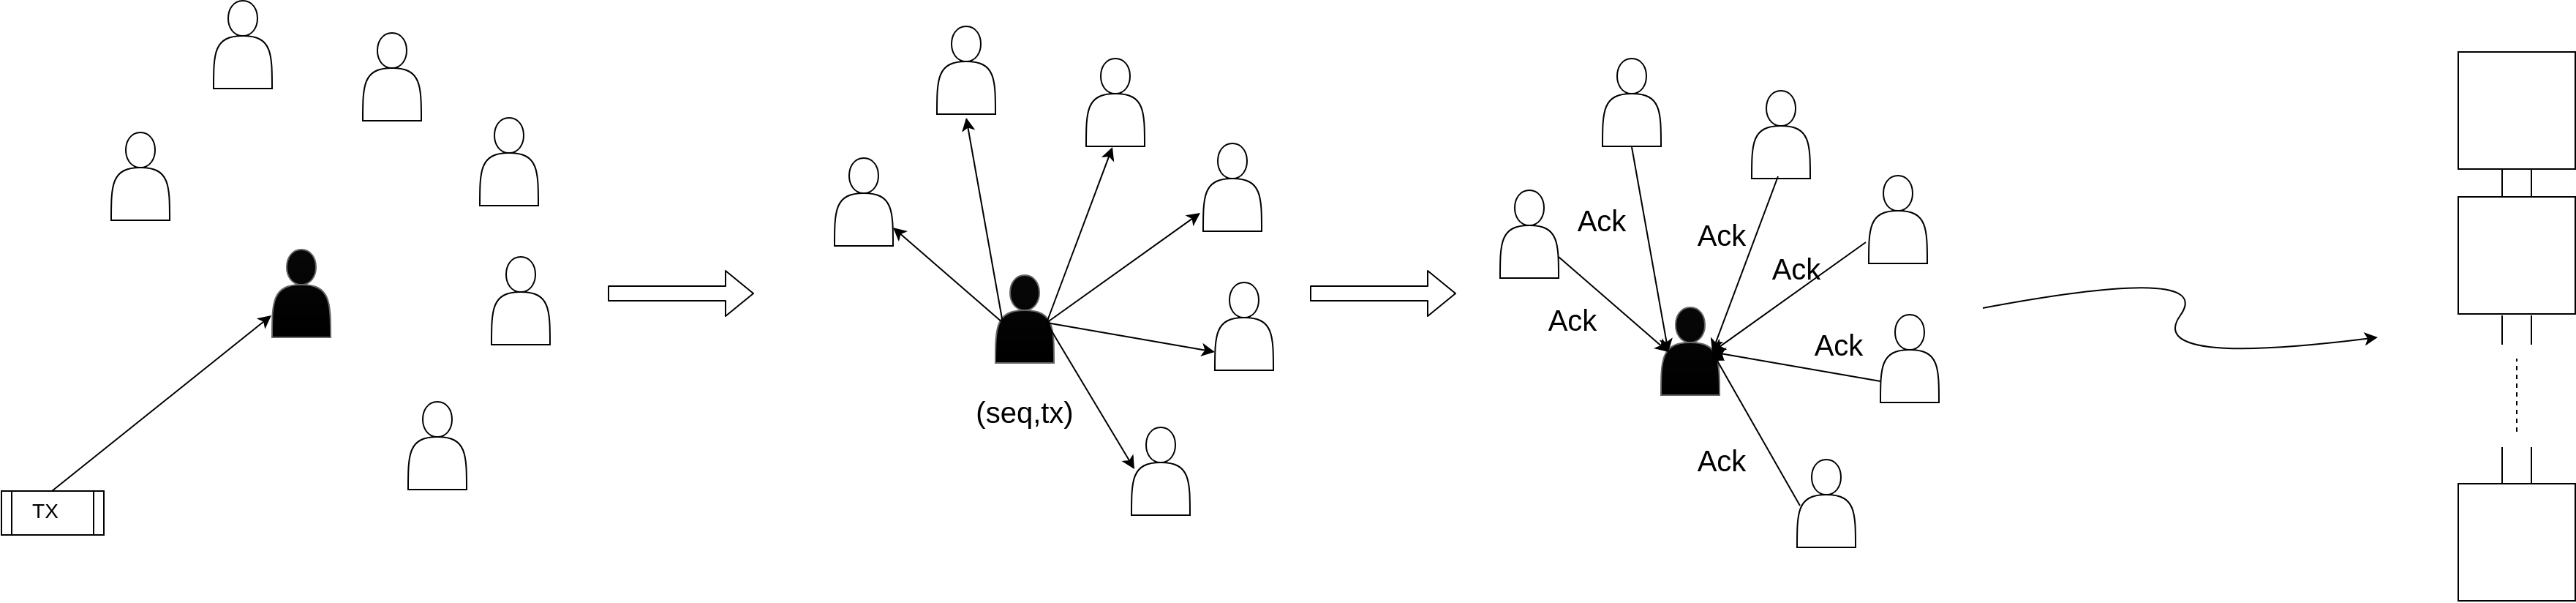
\includegraphics[width=\linewidth]{images/thunderella-design.png}
    \caption{Thunderella optimistic fast path}
    \label{fig:thunderella-design}
\end{figure}

Figure \ref{fig:thunderella-design}, provides an illustration of the Thunderella protocol. A user presents a transaction to the leader. The leader forwards the transaction to the committee along with a sequence number. The committee validates the transactions and checks the uniqueness of the sequence number. After validating the request, the committee responds with a signed \emph{ack}, which confirms the transaction. These transactions are gossiped to the underlying blockchain which includes the full view of the committee into the blockchain.

\subsection{Analysis}
First the model which sets the foundation for the analysis will be introduced, with further concreteness of the above mentioned protocol along with necessary primitives required for the analysis. This will be followed by the core theorems referenced in \cite{thunderella}, to show its security properties in the consensus protocol. 

\subsubsection{Model}

\cite{thunderella} adopts the standard \emph{Interactive Turing Machines} approach to model the execution of the protocol. The nodes, members of the committee and the leader, are activated by an environment $\mathcal{Z}(1^k)$, where $\kappa$ is the security parameter. The environment controls when nodes are spawned, corrupted, put to sleep, or woken up. If a node is corrupted, then it is controlled by the adversary $\mathcal{A}$, who can read all the input messages and set all the output messages of the given node. If a node is honest and sleeping, then it stops sending and receiving protocol messages, and furthermore it stops any computation with regard to the protocol. In the classical distributed systems terminology a sleeping node is considered corrupt, but in \cite{thunderella} an honest node effected by an outage is not considered as being controlled by the adversary. \cite{thunderella} considers this because, they want to prove that their Thunderella paradigm ensures consistency and worst-case liveness, whenever a fraction $\alpha$ of the committee are honest but can be asleep, while assuming the underlying blockchain is secure. When the environment $\mathcal{Z}$ decides to wake a node, the node comes back online and awaits the set of messages it should have received while asleep, in which adversarial messages can have been inserted. Furthermore, the environment $\mathcal{Z}$ has the possibility to kill a node controlled by the adversary, though the adversary will retain the \emph{view} of the corrupt node from before it was killed. For this analysis, the set \emph{online nodes} contain both honest nodes, which are not sleeping, and corrupted nodes, which have yet to be killed by the environment $\mathcal{Z}$. \\

The model uses round-based execution, meaning the protocol is executed in rounds, and at the beginning of each round the honest and online nodes receive inputs from the environment $\mathcal{Z}$, and at the end of a round they send their outputs to the environment $\mathcal{Z}$.\\


\paragraph{Communication} In the communication model, the adversary $\mathcal{A}$ has a lot of control over how messages are propagated; The adversary can reorder and delay messages sent by honest and online nodes, but cannot modify the contents. The adversary is allowed to send messages to a subset of honest and online nodes but not all of them. Though with respect to the delay imposed by the adversary, honest and online nodes can always send messages to the other honest and online nodes. The $\Delta$-bounded-delay is defined as: \\


\hfill\begin{minipage}{\dimexpr\textwidth-0.5cm}
Given a honest and online node sends a message $m$ at time $t$, then in any round $r \geq t + \Delta$, then any node online in round $r$ will receive the message $m$. This also includes nodes that may have been sleeping, but woke up or spawned in round $r$.
\end{minipage} \\


\noindent It is said that $(\mathcal{A}, \mathcal{Z})$ respects $\Delta$-bounded-delay iff $\mathcal{Z}$ inputs $\Delta$ to all honest nodes when spawned.\\


There are certain constraints imposed on the execution of the environment $(\mathcal{A}, \mathcal{Z})$ which is used to show security. The constrained execution on the environment $(\mathcal{A}, \mathcal{Z})$ with regards to ($n,\rho,\Delta$) on some protocol $\Pi$, with the constraints that during each round there are exactly $n$ online nodes, among which most $\rho n$ are corrupt, that $(\mathcal{A}, \mathcal{Z})$ comply with the delay $\Delta$ and all nodes are informed of $(n, \rho, \Delta)$.

The corruption constraint in the static case, is that corrupt nodes are only allowed to be spawned as such by the environment. Honest nodes already spawned cannot be adaptively corrupted throughout the execution of the protocol.

% Section 2.2 State Machine Replication - Consistency
\paragraph{State machine replication} As \cite{thunderella} wants to achieve consensus like the ones described in the literature of the classical distributed systems, they seek to show the same two critical security properties; Consistency and liveness. Consistency focuses on that all honest nodes should agree on the same logs, while liveness focuses on that issued transactions will quickly be included. \cite{thunderella} also employs the notion $LOG$ to describe the output collected thus far to the environment $\mathcal{Z}$. 
More formally, the definition of consistency and liveness are as follows:

\begin{itemize}
    \item \textbf{Consistency} A view of a node satisfies consistency iff the following hold:
    \begin{itemize}
        \item \textbf{Common prefix} A $LOG$ and $LOG'$ output to $\mathcal{Z}$ by two honest nodes $i$ and $j$ at time $t$ and $t'$, it must hold that $LOG \preceq LOG'$ or $LOG' \preceq LOG$. With $\preceq$ denoting the prefix-relationship between two $LOG$s.
        \item \textbf{self-consistency} An honest and online node $i$ will always output self-consistent logs, s.t., given a $LOG$ output at time $t$ and a $LOG'$ at time $t' \geq t$, then it holds that $LOG \preceq LOG'$.
    \end{itemize}
    \item \textbf{Liveness} A view satisfies $(T_\text{confirm},T_\text{warmup})$-liveness, where $T_\text{confirm}$ and $T_\text{warmup}$ are polynomial functions in the security parameter $\kappa$ provided by $\mathcal{Z}$ as input, iff the following holds: If some honest and online nodes in a round $T_\text{warmup} < t \leq |view|-T_\text{confirm}$ either received an input set $txs$ that contains some transaction $m$ from $\mathcal{Z}$ or that it has $m$ in its output log to $\mathcal{Z}$, then for any honest and online node at time $t^{'} \geq t+T_\text{confirm}$, $m$ would be contained in their output log.
\end{itemize}

% Blockchain
\paragraph{Underlying blockchain technology} \cite{thunderella} utilizes an underlying blockchain technology as their fallback mechanism for when either the leader or the committee is acting maliciously or is down. Therefore, \cite{thunderella} wants to create an abstraction to the the concrete instantiation of the blockchain, by simply stating that the underlying blockchain must satisfy \emph{chain growth}, \emph{chain quality} and \emph{consistency}. These three properties are described and proved for the systems in chapter \ref{cha:pow} and \ref{cha:pos}, where \emph{consistency} substitutes the \emph{common prefix} property. Following the three properties, \cite{thunderella} states that such a block-chain also implies a state machine replication. The underlying block-chain that the Thunderella protocol is based on is the Proof-of-Work model, but \emph{should} hold for any blockchain satisfying the three mentioned properties.\\

% Chain-State function
Given the abstract blockchain, an efficient chain-state function $\Gamma$ exists. $\Gamma$ divides the chain into multiple epochs interspersed with interim blocks. Blocks that are not attached to an epoch are called interim blocks. Every epoch always contains two sub-phases, an \emph{optimistic period} and a \emph{grace period} which both contain $\kappa$ blocks, resulting in an epoch always consisting of $2\kappa$ consecutive blocks.
$\Gamma(\kappa, \cdot, \cdot)$ is a chain-state function iff $\Gamma(\kappa, chain, \ell)$, for any chain and $0 \leq \ell \leq |chain|$ outputs one of the following:
\begin{itemize}
    \item ($e, optimistic$): chain[$\ell$] being an optimistic block
    \item ($e, grace$) chain[$\ell$] being a grace block
    \item $interim$: chain[$\ell$] being an interim block
\end{itemize}

\cite{thunderella} additionally denotes that the chain-state function $\Gamma(\kappa, \cdot, \cdot)$ is admissible if for any chain the following hold:
\begin{itemize}
    \item For any $0 \leq \ell \leq \ell' \leq |chain|$, if chain[$\ell$] belongs to epoch $e$ and chain[$\ell'$] belongs to epoch $e'$ then $e \leq e'$.
    \item For every epoch $e$, the optimistic blocks must appear consecutively and before the grace blocks.
    \item For every epoch $e$, there must be at least $\kappa$ grace blocks unless it is the end of the chain.
    \item For every $0 \leq \ell \leq |chain|$, then $\Gamma(\kappa, chain, \ell)$ depends only on chain[$:\ell$].
\end{itemize}


\subsubsection*{Formal protocol}


Before showing consistency and worst-case liveness for the Thunderella protocol, a few definitions, namely \emph{lucky sequence}, \emph{linearize}, and the core protocol for consistency $\Pi_{\text{thunder}}$ will need an introduction.\\

% Notarized transactions
A notarized transaction is a tuple $(e, s, m, V)$, where $e$ is the epoch, $s$ is the sequence number, $m$ is the message, and $V$ contains a signature along with the public keys of all committee members, that have signed this transaction, i.e., $\{(pk_i, \sigma_i) \; | \; \forall \; i \in committee\}$. It follows that $|V| \geq \frac{3}{4} \cdot |committee|$. A sequence of notarized transactions, \\ $\{(e_i, s_i, m_i, V_i)\}_{i \in [m]}$, is a lucky sequence iff for all $i \in [m]$ holds that $e_i = e$ and $s_i = i$. Additionally, a \emph{strip} function is used on transactions, which simply discards the the signatures and public keys of a transaction if present. I.e., strip($e, s, m, V$) = $(e, s, m)$, while unnotarized transactions are unchanged, $strip(m) = m$. \\


% Linearize
A \emph{linearize} function, denoted $linearize^{\Gamma(\kappa, \cdot, \cdot)}(chain)$ and often simplified to $linearize(chain)$, is defined to simplify the output of the transactions of the blockchain. 
\begin{enumerate}
    \item For each epoch e chain[$\ell: \ell'$] output:
    \begin{itemize}
        \item Extract the maximal lucky sequence $TXs$ from chain[$:\ell'$] in epoch $e$, and output Strip($TXs$).
        \item If chain[$l$] is not the end of the chain, let $TXs'$ be all remaining records in chain[$\ell:\ell'$] not contained in TXs, output Strip($TXs'$)
    \end{itemize}
    \item For each interim chain[$\ell : \ell'$] extract all transactions $TXs$ and output Strip($TXs$). 
\end{enumerate}

The core protocol for consistency $\Pi_\text{thunder}^{\Gamma(\kappa, \cdot, \cdot)}$, which are parametrized by the admissible chain-state function, in \cite{thunderella} is described in the following way.

\begin{itemize}
    \item \textbf{Initialize}:
    \begin{itemize}
        \item Call $(pk,sk) \xleftarrow{} \Sigma.\text{Gen}(k)$ to generate a signing key pair. Output $pk$ to $\mathcal{Z}$.
        \item Wait to receive committee from $\mathcal{Z}$, and henceforth, validity of votes and acceptability of chains will be defined with respect to committee.
        \item Fork an instance of the $\Pi_\text{blockchain}$ protocol with appropriate parameters determined by $\rho, n$ and $\Delta$.
    \end{itemize}
    
    \item \textbf{Notarize}: Upon receiving a notarization request $(e,s,m)$ from $\mathcal{Z}$: if $pk \in \text{committee}$ and no signature has been produced for $(e,s)$ earlier, compute $\sigma := \Sigma.\text{Sign}_{sk}(e,s,m)$ and broadcast $((e,s,m),\sigma)$.
    
    \item \textbf{Propose}: Every round, let chain be the output from the $\Pi_\text{blockchain}$ instance.
    \begin{itemize}
        \item Let $TXs$ be a set containing 1) every notarized transaction $(e,s,m,V)$ in the node's view such that no notarized transaction $(e,s,m,_)$ has appeared in $\text{chain}[:-0.5\kappa]$; and 2) every unnotarized transaction $m$ in the node's view such that no $m$ or notarized transaction $(e,s,m,\_)$ has appeared in $\text{chain}[:-0.5\kappa]$.
        \item Propose $TXs$ to $\Pi_\text{blockchain}$.
    \end{itemize}
    
    \item \textbf{Output}: In every round, let chain be the output from $\Pi_\text{blockchain}$.
    \begin{itemize}
        \item If $\text{chain}[-0.5\kappa]$ is an optimistic block belonging to epoch $e$, then
        \begin{enumerate}
            \item Let $\text{chain}[-\ell]$ be the starting block for epoch $e$ in chain where $\ell \geq 0.5\kappa$.
            \item Extract the maximal lucky sequence $TXs$ for epoch $e$ from the node's view so far.
            \item Let $\overline{LOG} := \text{linearize}(\text{chain}[:-(\ell+1)])||strip(TXs)$.
        \end{enumerate}
        \item Else, let $\overline{LOG} := \text{linearize}(\text{chain}[:-0.5\kappa])$.
        \item Let $LOG$ be the previous output to $\mathcal{Z}$: If $\overline{LOG}$ is longer than $LOG$, then output $\overline{LOG}$, else output $LOG$ to $\mathcal{Z}$.
    \end{itemize}
    
    \item \textbf{Mempool}: Upon receiving any other message from the network or $\mathcal{Z}$, record the tuple.
\end{itemize}


\subsubsection*{Consistency and worst-case liveness}

Theorems for consistency and worst-case liveness will be covered in this section as well as their respective proofs.\\

Fact 4 from \cite{thunderella} is used in both proofs, and is therefore mentioned below.
\begin{fact}
For any chain and any $0 \leq i < j \leq |\text{chain}|$, $\text{linearize}^{\Gamma(\kappa,\cdot,\cdot)}(\text{chain}[:i]) \preceq \text{linearize}^{\Gamma(\kappa,\cdot,\cdot)}(\text{chain}[:j])$, when $\Gamma(\kappa,\cdot,\cdot)$ is any admissible chain-state function.
\end{fact}


\begin{theorem}[Consistency]
\label{th:thunder-consistency}
Let $\Gamma(\kappa, \cdot, \cdot)$ be any admissible chain-state function. Then $\Pi_{\text{thunder}}^{\Gamma(\kappa, \cdot, \cdot)}$ satisfies consistency with respect to any p.p.t. $(\mathcal{A}, \mathcal{Z})$ that is compliant with respect to $\Pi_{\text{thunder}}^{\Gamma(\kappa, \cdot, \cdot)}$.
\end{theorem}

To prove theorem \ref{th:thunder-consistency}, \cite{thunderella} firstly notes that the output $LOG$ of an honest node never shrinks, due to the construction of the protocol. Second, the common prefix and future self-consistency follows from honest nodes following the protocol and the following lemma.

% lemma used to prove consistency theorem
\begin{lemma}
Let $\Gamma(\kappa, \cdot, \cdot)$ be any admissible chain-state function. Except with negligible probability over the choice of \textbf{view}, the following holds: For any $r$ and $t$, for any node $i$ honest and online in round $r$ and any node $j$ honest and online in round $t$, either $\overline{LOG}_i^r \prec \overline{LOG}_j^t$ or $\overline{LOG}_j^t \prec \overline{LOG}_i^r$.
\end{lemma}

To prove this lemma, \cite{thunderella} considers two logs on the following form 
\begin{align*}
    \overline{LOG}^r_i &= \text{linearize}(\text{chain}_i^r[:-\ell])||\text{strip}(TXs) \\
    \overline{LOG}^t_j &= \text{linearize}(\text{chain}_j^t[:-\ell'])||\text{strip}(TXs')
\end{align*}

Here $TXs$ is either empty and $\ell,\ell^{'} = 0.5\kappa$ or $TXs$ contains a lucky sequence over an epoch and $\ell,\ell^{'} \geq 0.5\kappa$. The $BAD$ event is ignored by \cite{thunderella} for the remainder of the proof, since it only happens in a negligible fraction of the views. For the rest of the views, it is stated that either $\text{chain}_i^r[:-\ell] \preceq \text{chain}_j^t[:-\ell^{'}]$ or $\text{chain}_j^t[:-\ell^{'}] \preceq \text{chain}_i^r[:-\ell]$, which is due to consistency assumption of the underlying blockchain protocol. It is assumed that $\text{chain}_i^r[:-\ell] \preceq \text{chain}_j^t[:-\ell^{'}]$, which can be done without loss of generality. 

Since the $TXs$ can be both empty and non-empty, \cite{thunderella} consideres both as seperate cases.\\

In \textbf{case 1} the $TXs$ is considered to be empty, then $\text{chain}_i^r[:-\ell] \preceq \text{chain}_j^t[:-\ell^{'}]$ follows from the fact stated previously.\\

In \textbf{case 2}, the $TXs$ is considered to be non-empty and thereby it would contain a lucky sequence for some epoch $e$. $\text{chain}_i^r[-\ell]$ will be the starting block for $e$ and $\text{chain}_i^r[-0.5\kappa]$ is an optimistic block of $e$. \cite{thunderella} considers two sub-cases, one where $e$ has completed in $\text{chain}_j^t[:-\ell^{'}]$ and another where $e$ has not completed in $\text{chain}_j^t[:-\ell^{'}]$.

In \textbf{case 2.1}, the last block of $e$ in $\text{chain}_j^t[:-\ell^{'}]$ is denoted $\text{chain}_j^t[:-\ell^{*}]$. From the aforementioned fact, it holds that
\begin{equation*}
    \text{linearize}(\text{chain}_i^r[:-\ell])||\text{strip}(TXs) \preceq \text{linearize}(\text{chain}_j^t[:-\ell^{*}])
\end{equation*}
$TXs$ is the lucky sequence for $e$ in the view of an honest node $i$ in round $r$, then by $r+\Delta$, the $TXs$ must be contained in the view of any honest nodes. $\text{chain}^t_j[:-\ell^{*}]$ will have to be at least $0.5k$ longer than $\text{chain}^r_i$, which is due to the chain-state function $\Gamma$ being admissible (item 2 and 3 of the definition) and $\text{chain}^r_i[-0.5\kappa]$ being an optimistic block. At round $r+\Delta$ any honest chain will have a length at most $|\text{chain}^r_i|+0.25\kappa$, this is due to the \emph{growth upper bound} on $(T,g_0,g_1)$-\emph{chain growth}, which states that $|\text{chain}^t|-|\text{chain}^r| \leq \lceil g_1(t-r) \rceil$. Furthermore, a lucky sequence of length $|TXs|$ within the epoch $e$ will have to be contained in $\text{chain}^t_j[.-\ell^{*}]$, which is due to the liveness property. The rest of this case follows from lemma 2 in \cite{thunderella}, which states: \emph{For any $(e, s)$ pair, if two notarized transactions ($e,s,m, V$), ($e, s, m', V'$) appear in a view, then it must be $m=m'$}, and the definition of \emph{linearize}.

In \textbf{case 2.2}, the $chain^t_j[-\ell']$ has not completed epoch $e$. From the protocol, each node $i$ will output $linearize(chain^r_i[:-\ell])||strip(TXs)$ in round $r$. Now given that $linearize(chain^r_i[:-\ell]) \preceq linearize(chain^t_j[:-\ell'])$ from the honest protocol, it follows that node $j$'s view must be of the type $linearize(chain^r_i[:-\ell])||strip(TXs^*)$ where node $j$'s transactions $TXs^*$ is either empty or a lucky sequence. From \cite{thunderella}'s lemma 2, it follows that $\overline{LOG^r_i} \preceq \overline{LOG^t_j}$, and since the assumption that $chain^r_i[:-\ell] \preceq chain^t_j[:-\ell']$ is without loss of generality it can also be extended to $\overline{LOG^t_j} \preceq \overline{LOG^r_i}$. \\

For showing the \emph{worst-case liveness} an initial lemma will be introduced and and argued for followed by the theorem showing the worst-case liveness property.

% Lemma 4
\begin{lemma}[Worst-case liveness variant]
Let $\Gamma^{pred}(\kappa, \cdot, \cdot)$ be the chain-state function for an arbitrary polynomial-time next-epoch function $pred$. Let $g_0$ denote the underlying $\Pi_{blockchain}$'s chain growth lower bound parameter. Except with negligible probability over the choice of $view$, the following holds: Suppose that $\mathcal{Z}$ inputs a transaction $m$ to an honest node when its $chain$ output from $\Pi_{blockchain}$ has length $\ell$, then for any honest chain $chain'$ in $view$ of length at least $\ell + 2.5\kappa$, it must hold that $m$ or some ($\_,\_,m$) exists in $linearize^{\Gamma(\kappa,\cdot,\cdot)}(chain'[:\ell+2.5\kappa])$.
\end{lemma}

The liveness of the underlying blockchain $\Pi_{blockchain}$, guarantees that either $m$ or some tuple ($\_,\_,m,\_$) is included by $chain'[:\ell+0.25\kappa]$. $chain'[\ell_0]$ is defined to be the time when $m$ was included, with $\ell_0 \leq \ell+0.25\kappa$. Thus two cases can occur: 
\begin{itemize}
    \item $chain'[\ell_0]$ is an interim block. From linearize it is defined that all interim blocks, it will output strip($m$). Thus the transaction $m$ will be included at $chain'[\ell_0]$, and since $\ell_0 \leq \ell+1$ it follows from the fact stated previously, that
    \begin{equation*}
        \text{linearize}^{\Gamma(\kappa,\cdot,\cdot)}(\text{chain}[:\ell_0]) \preceq \text{linearize}^{\Gamma(\kappa,\cdot,\cdot)}(\text{chain}[:\ell+1])
    \end{equation*}
    
    \item $chain'[\ell_0]$ belongs to an epoch $e$. From $\Gamma$ if $linearize(chain'[l_0+\kappa])$ does not contain $m$, the chain will enter the grace period, which has a length of $\ell_0 + \kappa + 1$ or smaller. Each epoch lasts at maximum $2\kappa$, and as such the message will be on the chain at $\ell_0 + 2\kappa < \ell + 2.5\kappa$. As such the message $m$ will be included in at least $linearize(chain'[:\ell + 2.5\kappa])$.
\end{itemize}



\begin{theorem}[worst-case liveness]
Let $\Gamma(\kappa, \cdot, \cdot)$ be the chain-state function. Let $g_0$ denote the underlying $\Pi_{blockchain}$'s chain growth lower bound parameter, and let $T_{confirm}(\kappa) := \frac{3\kappa}{g_0}$. For any p.p.t. ($\mathcal{A}, \mathcal{Z}$) that is compliant w.r.t $\Pi_{thunder}^{\Gamma(\kappa, \cdot, \cdot)}$ there exists a negligible function $negl(\cdot)$ such that for every $\kappa \in \mathbb{N}$, except with $negl(\kappa)$ probability over the choice of $view \xleftarrow{} EXEC^{\Pi_{thunder}^{\Gamma(\kappa, \cdot, \cdot)}}(\mathcal{A}, \mathcal{Z}, \kappa)$, the following holds: suppose that $\mathcal{Z}$ inputs a transaction $m$ to an honest node in round $r$, then in any round $r' \geq r + T_{confirm}(\kappa)$, all honest and online nodes output $LOG$ to $\mathcal{Z}$ will contain some ($\_,\_,m$) or $m$
\end{theorem}

In a round $r$, with the longest honest chain of length $\ell_r$, it follows from the \emph{worst-case liveness variant} lemma and from the previously stated fact, that any honest chain in view with a length of at least $\ell_r + 3\kappa$, must contain the transaction $m$ in $linearize(chain[: -0.5\kappa])$. From round $r+T_\text{confirm}$ and ahead, it follows that $chain'$ of every honest node must be of length at least $\ell_r + 3\kappa$, due to the lower bound on the chain growth of the underlying blockchain. This results in the transaction $m$ being contained in the prefix of the $LOG$ for any $chain'$, with $LOG$ being the output to the environment for the round, which follows from the corollary in \cite{thunderella}: 

% Corollary 3 used for the remainder of the proof of liveness
\begin{corollary}
Let $\Gamma(\kappa, \cdot, \cdot)$ be any admissible chain-state function. Except with negligible probability over the choice of \textbf{view}, the following holds: For any round $r$, for any node $i$ honest and online in round $r$, $\text{linearize}(\text{chain}^r_i[:-0.5\kappa])$ is a prefix of $LOG_i^r$ where $\text{chain}_i^r$ is node $i$'s $\Pi_\text{blockchain}$ output in round $r$, and $LOG_i^r$ is node $i$'s output log to $\mathcal{Z}$ in round $r$.
\end{corollary}

\subsubsection*{Permissionless Extension}
% is this peer?
The outlined protocol assumes that there exists a static stake. To not have such dedicated trusted peers, the permissionless blockchain will want to be able to elect new committees and leaders over time during the execution of the protocol.

% how the protocol is extended

For the protocol to be extended to a permissionless setting, \cite{thunderella} modifies \emph{lucky sequence}, \emph{chain linearization} and the \emph{core protocol for consistency} $\overset{\sim}{\Pi}_\text{thunder}$. Firstly, a transaction is denoted $(e,s,c,c',m,V)$, where $c$ denotes the clock number for the current transaction and $c'$ denotes the intended clock number for the next transaction. For the lucky sequence, \cite{thunderella} additionally assumes, that an epoch number is a tuple containing the epoch number and the starting clock number. For the chain linearization, a transaction can be legitimately included in the chain in clock interval $[c, c+2\kappa]$, further the \emph{strip}-function used in chain linearization will reduce a transaction to $(e,s,c,c',m)$. 

For the modified protocol $\overset{\sim}{\Pi}_\text{thunder}$, a \emph{committee selection} has been included right after the \emph{initialization}. In the \emph{committee selection}, when receiving $\text{elect}(c,\text{committee}_c)$ from $\mathcal{Z}$, $\text{committee}_c$ is recorded for clock $c$. In the \emph{propose} phase, a node previously proposed a $TXs$ to $\mathcal{Z}$, but in the modified protocol, the node will propose $TXs||pk$ such that $\mathcal{Z}$ can choose a committee based on the observed public keys. In the \emph{output phase}, when an optimistic block belongs to an epoch $e$, the node will from its view extract the maximal lucky sequence $TXs$ for $e$ as previously. Though, in case the next block enters the grace period, the clock number must be large enough for the notarized transaction to be picked up by the grace period.

Due to the modifications of \emph{lucky sequence}, \emph{chain linearization} and the \emph{core protocol for consistency} $\overset{\sim}{\Pi}_\text{thunder}$, the proofs of the theorems and lemmas for \emph{consistency} and \emph{worst-case liveness} are changed with respect to these modifications, though the theorems and lemmas are still the same.

% the two types

The above extensions provide a general framework for extending the static committee to a dynamic committee, but which policy to employ for selecting the committee still needs to be addressed. In the design section of the protocol two ways were described, namely the recent miners as the committee or stakeholders as committee. These were described informally which will be explained a bit more in depth here.

\paragraph{Miners as committee} Here it is assumed the underlying block-chain is a Proof-of-Work blockchain for selecting the committee. \cite{thunderella} references a different protocol called fruitchains \cite{fruitchains}. \cite{fruitchains} states that given any blockchain protocol, if the adversary controls at most $\rho$ fraction of corrupt nodes, then he will not be able to increase his representation by more than any small fraction $\epsilon$. So the protocol can pick the miners of the last $\kappa$ blocks, potentially removing some blocks that have not stabilized yet. Whenever a miner mines a block, a so-called "fruit" containing the public-key of the miner will be included, which is then used in the committee. \cite{thunderella} uses the result of the fruitchains paper, \cite{fruitchains}, as a blackbox for showing that given a good "fruit-quality" in the beginning of the protocol, it will remain as such. It should be noted that the security model is relaxed by not supporting fully adaptive corruptions, but only covers mildly adaptive corruptions, in which corruptions occur after a delay.

\paragraph{Stakeholders as committee} Having a Proof-of-Work or Proof-of-Stake chain, it may make sense to select the committee based on the stakeholders within the system. But given the Proof-of-Stake protocol, the stakeholders will need to serve two purposes; Generating blocks and validating transactions as a committee. \cite{thunderella} makes notes that having both responsibilities can be damaging to the consensus protocol. I.e., if the stakeholder sells his stake resulting in not having any incentive to act honestly throughout the term as a committee. \cite{thunderella} proposes two ways to solve this:
\begin{itemize}
    \item During a term, the stakeholders liquidity of the cryptocurrency will be limited.
    \item By having the committee members put down collateral. If they misbehave, then they lose their collateral.
\end{itemize}

No formal presentation of how this is done in \cite{thunderella}, but intuitively selecting either the $k$ biggest stakeholders or randomly selecting $p$ of $k$ stakeholders above \emph{some} stake threshold. The committee has the incentive of behaving honestly, otherwise their offered collateral is taken and the rewards for participating in the committee is lost. While potentially also negatively impacting the value of the cryptocurrency.


\subsection{Discussion}
\label{subsec:thunder-discussion}

% Framework on top of the existing

The Thunderella protocol is a framework, that is not reliant on any concrete instanciation of the underlying blockchain. As previously stated, it suits both the Proof-of-Stake or Proof-of-Work type block-chains with the assumption that they fulfil the chain-growth, chain-quality as well as the consistency property. \cite{thunderella} does a nice job of abstracting this into a so-called \emph{abstract blockchain}, such that the consensus protocol provided is not reliant on any concrete instanciation of these. As described in the analysis of Bitcoin, one of the core issues is that a block is only created once every 10 minutes  \cite{bitcoin-scalability}. This leads to a major bottle-neck in terms of how fast transactions can be approved, as well as driving transaction fees up as there is only room for a limited amount of transactions per block. Thunderella does provide a solution to the speed of which transactions can be confirmed, but some modifications to the original underlying chain is required.\\

% Adds more complexity to the underlying protocol by having to save a state constantly on the chain, while they do provide some arguements that these things can be pruned to be minimal
For the added amount of transactions, there needs to be a "special" data slot on the chain. This data slot will contain the transactions and states of the committee, who are validated by the Thunderella blockchain. Though  \cite{thunderella} does mention, that pruning the content of these can be done in order to keep the meta-data required for the protocol to a minimum. This still means that some current restrictions and changes to blocks are required for the Thunderella protocol to function, like removing the upper-bound of the amount of transactions per block.\\

% Neat for practical usage going to store or quickly saving data etc, but does present collateral to store if something goes wrong in the underlying chain and the transaction is lost
Assuming that the underlying chain is extended with these properties, it can extend the original chain to have more practical usage. Despite not being a focus of the analysis in this thesis, \cite{thunderella} does provide proofs for having optimistic responsiveness in lucky epochs. Meaning that the speed of which transactions get accepted is only limited by the maximum network delay. This means, it, perhaps a bit optimistically, can be used for every day things, such as shopping or other every day requirements for transactional systems. This is of course in the optimistic case, and requires some heuristicly assumptions, that it is very rare that fallbacks to the original blockchain is required.\\


% Concerns about double spending
One concern that may become an issue in this protocol is that the abstraction does not cover both transactions being introduced to the underlying blockchain as well as the quorum simultaneously. But instead, the Thunderella protocol \cite{thunderella} models only the quorum showing the core consistency properties. This can create the following issue: A peer can introduce a transaction to the underlying blockchain and the quorum simultaneously. As the quorum accepts the transactions, since it is not contained within any block, a miner in the underlying blockchain generates a new block containing the transactions. This means the underlying blockchain has contained the new transactions, while the transaction approved by the quorum may not have been introduced yet. If the receiver optimistically approves this transaction, since it is approved by the quorum, the malicious peer has effectively double spent the money. This raises concerns of which of the transactions should be approved, i.e., should the quorums transactions trump transactions contained within the underlying blockchain. Alternatively, a solution to seperate the currency related to the quorum might have to be presented, but exactly a solution to solve this, as well as the severity of the problem, will be left as future work. It is noted that the above attack does assume some inconsistency between the underlying blockchain and the quorum, but it is considered reasonable that a quorum cannot effectively share a view with all of the miners in a permissionless setting, as well as problems concerning asynchrony might appear.


% Proofs are confusing, from the way they index stuff and their formulation can sometimes come across as kinda confusing, but in generally they have a good model description as well as good proofs, aswell as showing the proof for adaptive cases. One potential error noted in proof of consistency
In the proof for the lemma used in proving theorem \ref{th:thunder-consistency}, the starting block for some epoch $e$ was changed from the starting block used in \cite{thunderella}. The starting block used in \cite{thunderella} is $\text{chain}^r_i[-\ell+1]$, here it is fair to assume $\ell=0.5\kappa$ since $\ell \geq 0.5\kappa$. But due to an optimistic block for the epoch $e$ being indexed $\text{chain}^r_i[-0.5\kappa]$, the sequence of blocks for epoch $e$ is confusing. If looking at a general $\text{chain}=\{x_1, \dots, x_N\}$, then $\text{chain}^r_i[:-\ell] = \{x_1, \ldots, x_{N-\ell}\}$. The starting block for epoch $e$ would be $x_{N-\ell+1}=x_{N-0.5\kappa+1}$ and the optimistic block for $e$ would be $x_{N-0.5\kappa}$, which is located before the starting block for $e$ in $chain^r_i[:-\ell]$, meaning it would be either an interim block or a grace block. Due to this confusing indexing, the start block was changed according to the \emph{output phase} of the $\Pi_\text{thunder}$ protocol. In the output phase of $\Pi_\text{thunder}$ it is stated that: \emph{If $chain[-0.5\kappa]$ is an optimistic block belonging to epoch $e$, let $chain[-\ell]$ be the starting block for epoch $e$ where $\ell \geq 0.5\kappa$}, which lead to believe that $\text{chain}^r_i[-\ell+1]$ as a starting block was an error and the real starting block should be $chain[-\ell]$.

